% #########################################################################
% ##                      FITXER: presentacio.tex                        ##
% ##        Contingut: Presentació del TFM en format Beamer UAB         ##
% #########################################################################

\documentclass[mathserif, aspectratio=169]{beamer}
\usepackage{presentacio_format} % Estil personalitzat amb colors UAB

% --------------------------------------------------- %
%                  Informació de la presentació       %
% --------------------------------------------------- %
\title[Predicció temperatura amb ML]{Predicció de temperatura a curt termini amb \textit{machine learning}}
\author[Pau Rodrigo]{Pau Rodrigo Parés}
\institute[UAB, SMC]{Universitat Autònoma de Barcelona \\ Servei Meteorològic de Catalunya}
\date{Juliol 2025}
\titlegraphic{
  
\includegraphics[width=0.25\linewidth]{figures/logos/logo-uab.png} \hspace{1cm}
  
\includegraphics[width=0.25\linewidth]{figures/logos/meteocat_c.png}
}

% --------------------------------------------------- %
%                       Document                      %
% --------------------------------------------------- %
\begin{document}

% --- Portada --- %
\begin{frame}[plain]
  \titlepage
\end{frame}

% --- Cita inicial --- %
\begin{frame}
  \centering
  \large
  \textit{"All models are wrong, but some are useful."} \\
  --- George Box
\end{frame}

% === Introducció === %
\section{Introducció}

\begin{frame}{Context i motivació}
  \begin{itemize}
    \item Importància de la predicció meteorològica a curt termini.
    \item Alta demanda computacional dels models numèrics clàssics.
    \item Possible rol de mètodes d'aprenentatge automàtic.
  \end{itemize}
\end{frame}

\begin{frame}{Objectiu del treball}
  \begin{block}{Objectiu principal}
    Avaluar models \textbf{Markov}, \textbf{ARIMA/SARIMA} i \textbf{LSTM} per a la predicció de temperatura a curt termini, comparant-ne el rendiment i la viabilitat operativa.
  \end{block}
\end{frame}

% === Dades === %
\section{Dades}

\begin{frame}{Origen de les dades}
  \begin{itemize}
    \item Xarxa XEMA del SMC
    \item Estació: La Bonaigua
    \item Període: 1998--2024
    \item Resolució horària
  \end{itemize}
\end{frame}

\begin{frame}{Exemple de la sèrie temporal}
  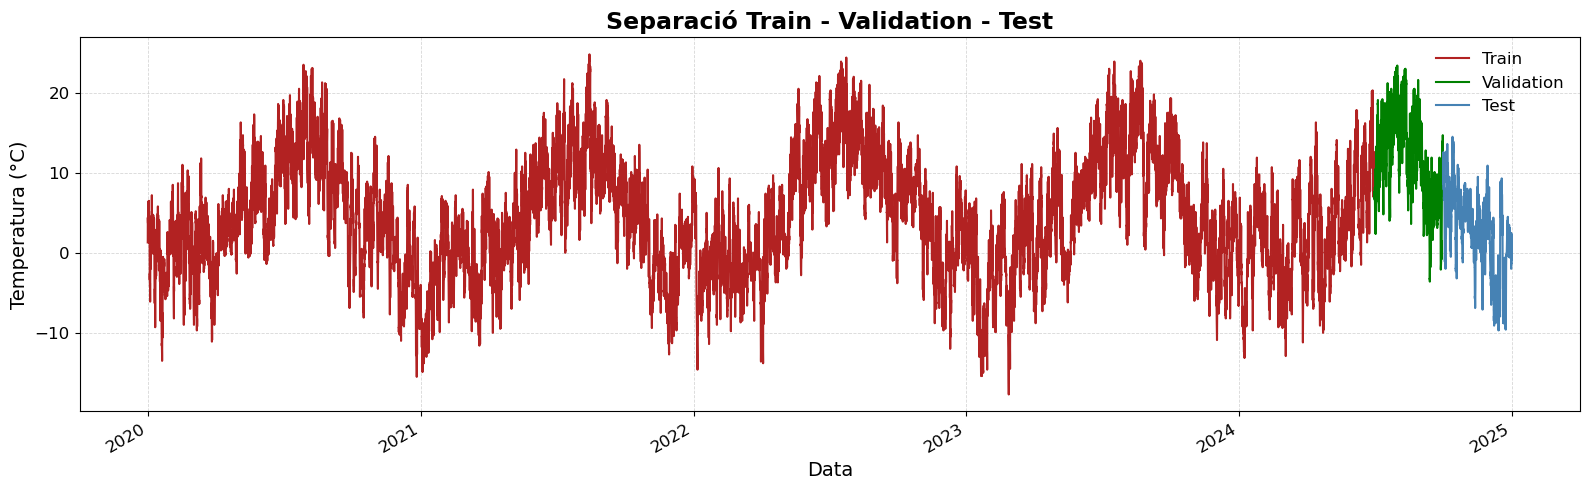
\includegraphics[width=\linewidth]{figures/lstm/data/data_splits_plot.png}
\end{frame}

% === Models === %
\section{Models}

\begin{frame}{Cadenes de Markov (precipitació)}
  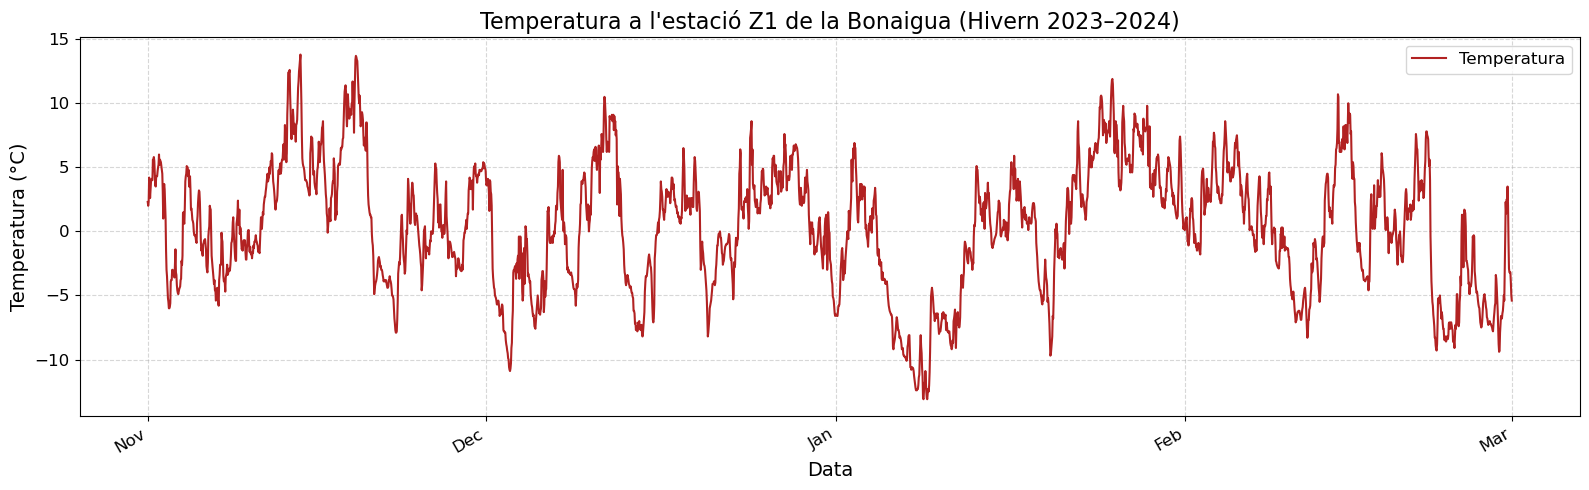
\includegraphics[width=0.9\linewidth]{figures/markov/1.png}
\end{frame}

\begin{frame}{Model ARIMA}
  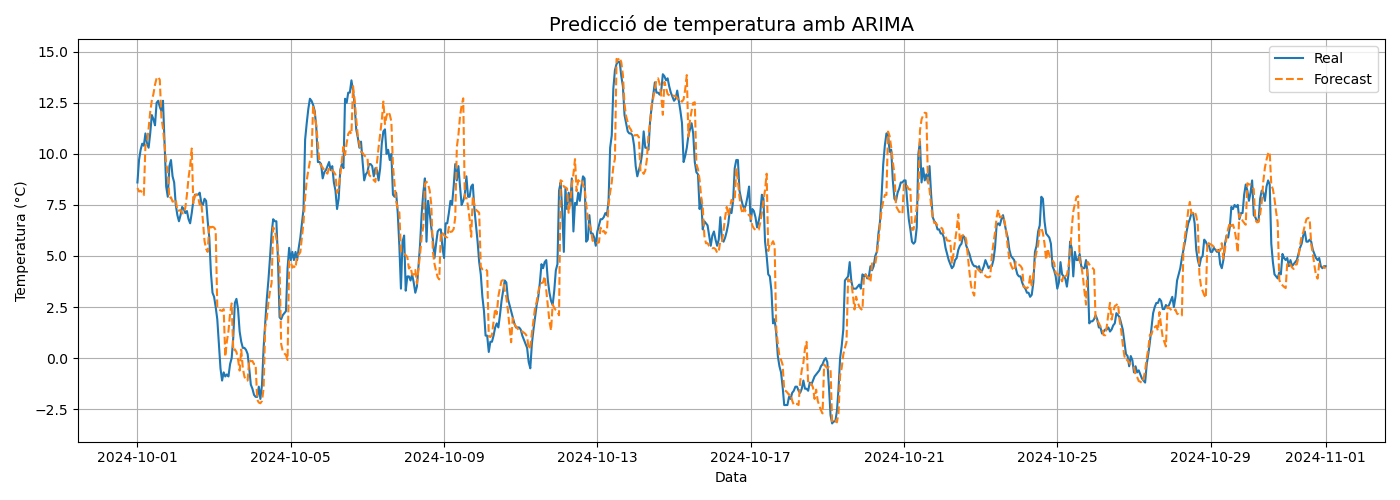
\includegraphics[width=0.9\linewidth]{figures/arima/C1_plot.png}
\end{frame}

\begin{frame}{Arquitectura LSTM}
  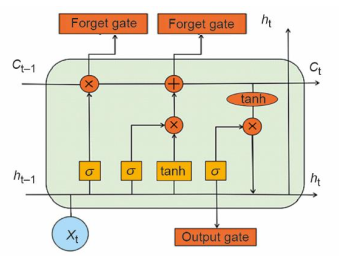
\includegraphics[width=0.9\linewidth]{figures/lstm/concept/1_lstm_cell.png}
\end{frame}

% === Resultats === %
\section{Resultats}

\begin{frame}{Comparació de models}
  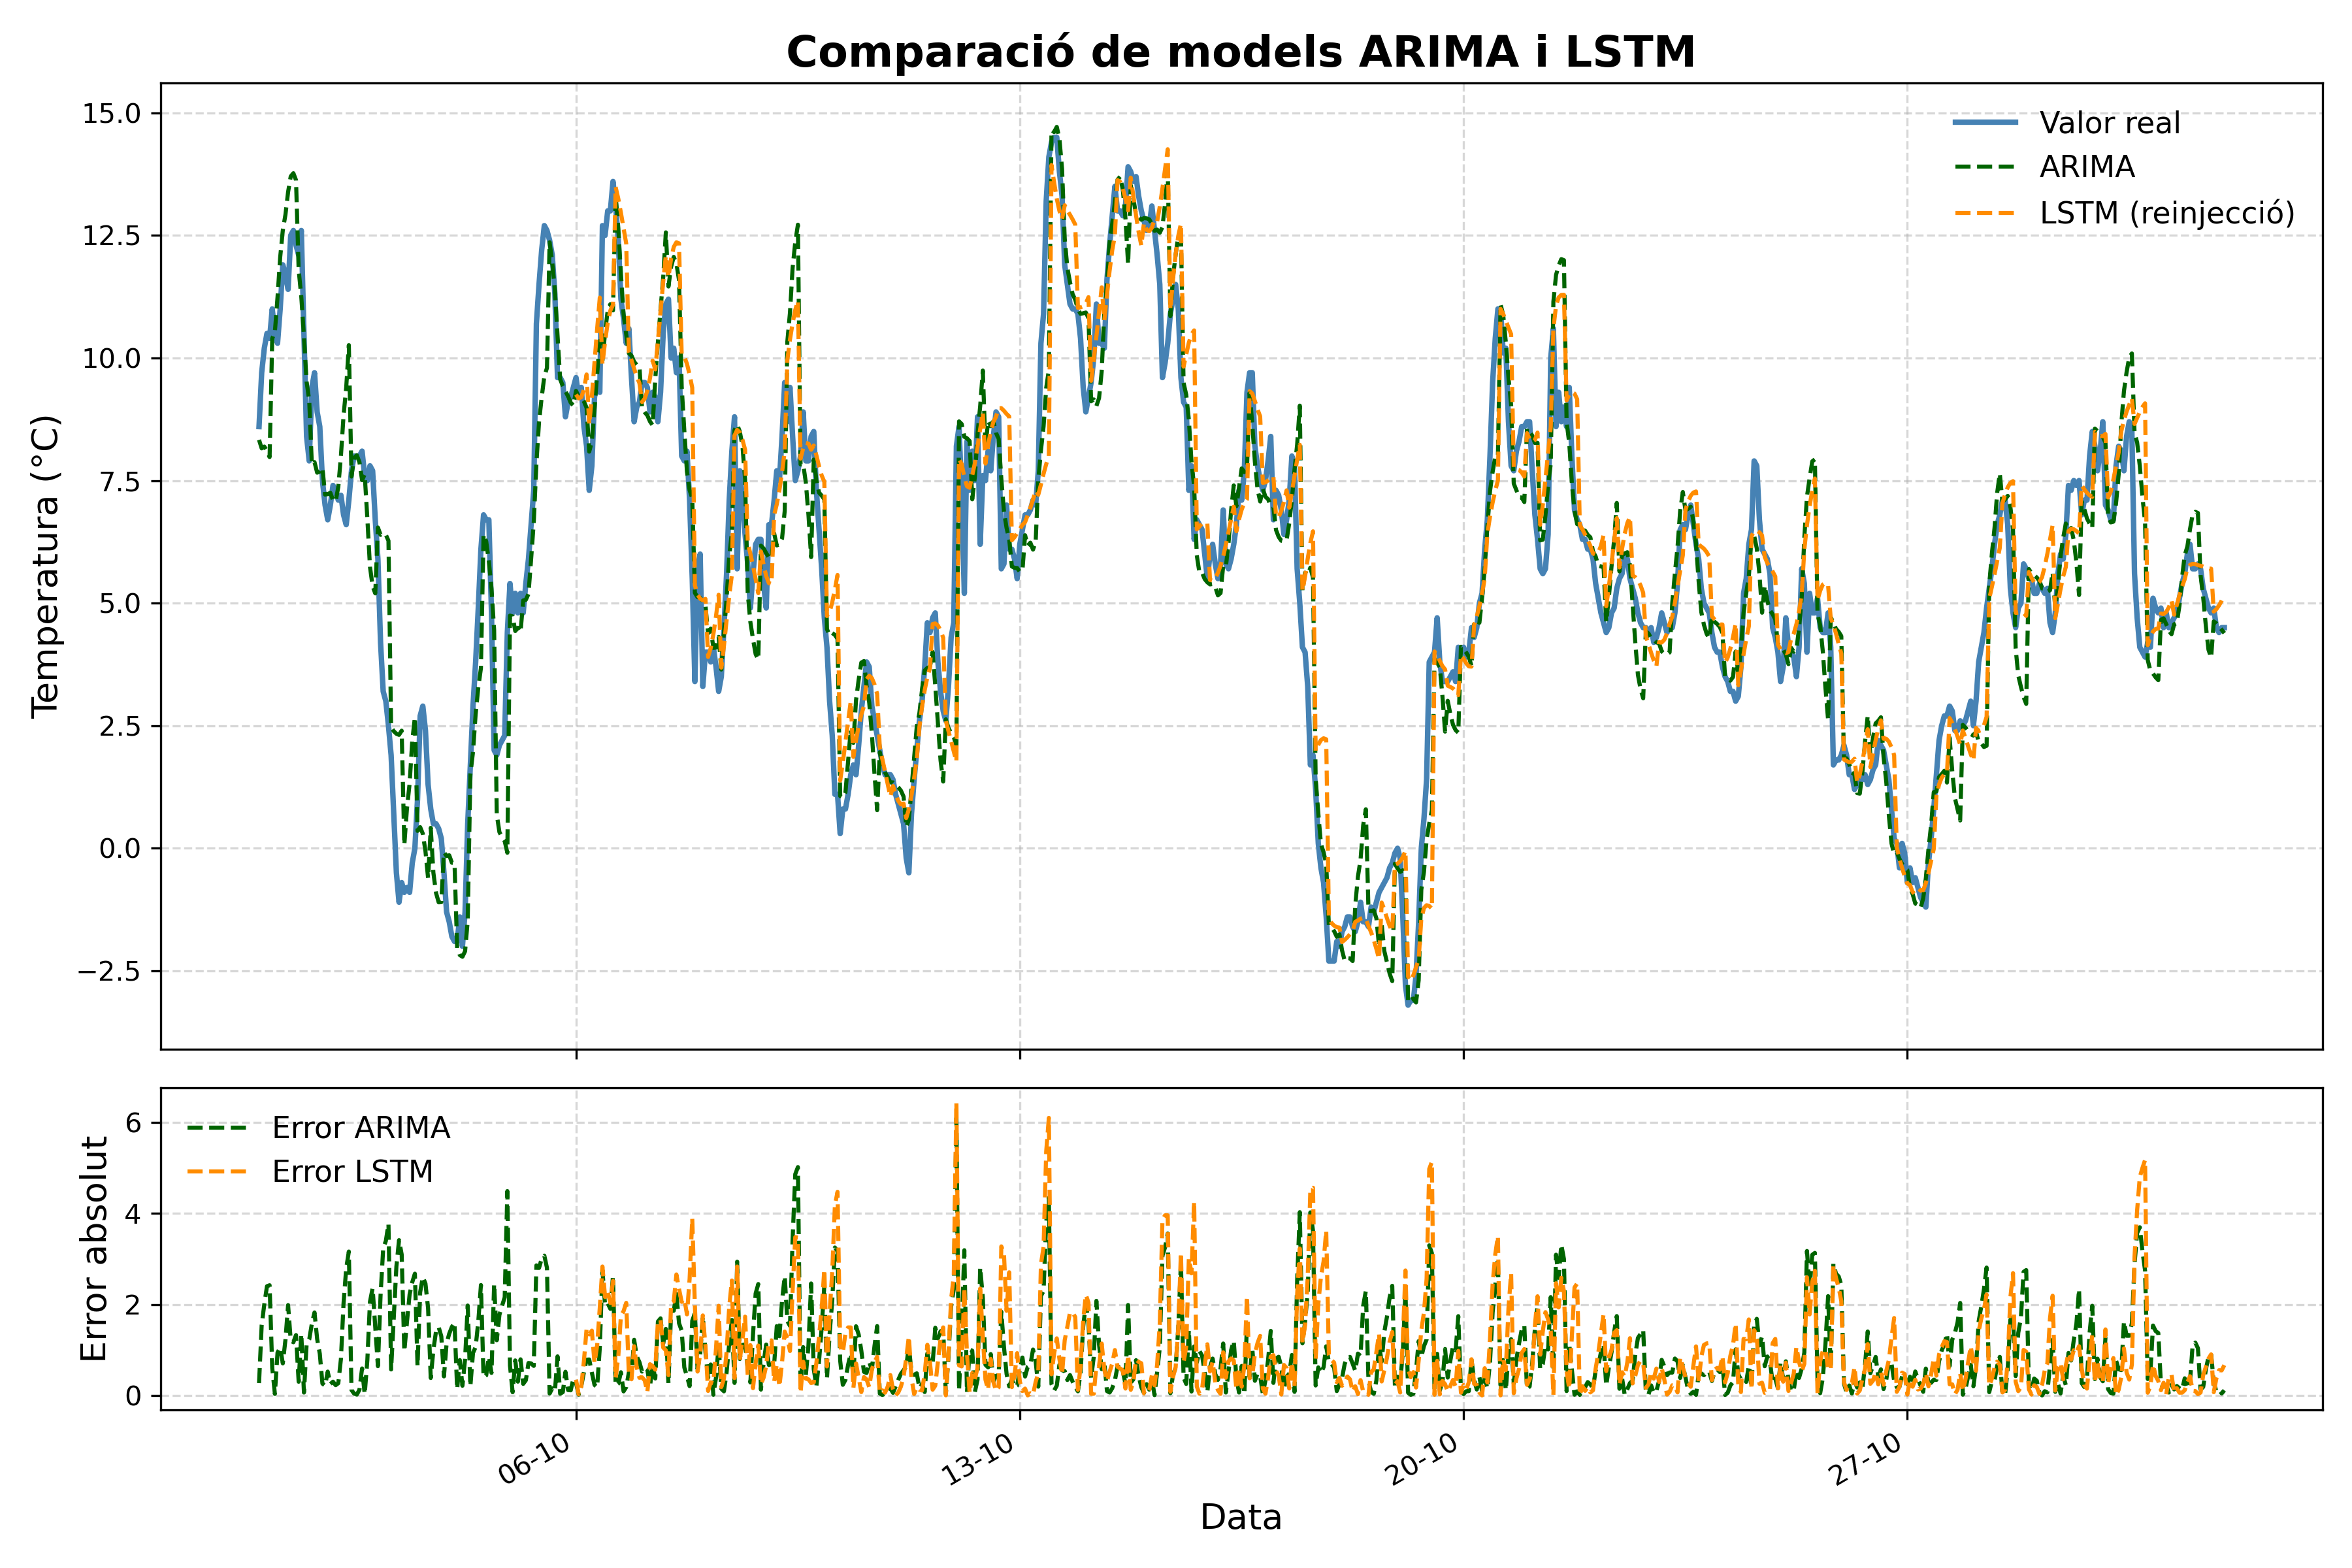
\includegraphics[width=0.95\linewidth]{figures/comp_arima_lstm/comparacio_models_amb_errors.png}
\end{frame}

% === Conclusions === %
\section{Conclusions}

\begin{frame}{Conclusions principals}
  \begin{itemize}
    \item ARIMA/SARIMA robustos a horitzons curts.
    \item LSTM milloren amb predicció iterativa i dataset gran.
    \item Models ML menys exigents computacionalment.
  \end{itemize}
\end{frame}

\begin{frame}{Limitacions i futur}
  \begin{itemize}
    \item Predicció operativa encara limitada (rolling forecast).
    \item Possibles millores amb models híbrids o ensemble.
    \item Ampliació a altres variables i estacions.
  \end{itemize}
\end{frame}

% --- Fi --- %
\begin{frame}[standout]
  Gràcies! \\
  \small Alguna pregunta?
\end{frame}

\end{document}
